\paragraph{Budget sufficiency and fixed-cost comparison.}

The development pilot is extended without changing its candidates, scores or execution rules. G attains 85.18\%, 93.38\% and 100\% coverage at budgets 256, 512 and 1024, respectively (Figure~\ref{fig:four-room-budget}). It first covers all free cells in the start-reachable reference at action 727 after 135.0 m; the complete 1024-action episode travels 189.6 m and returns without collision or false occupied labels on that reference. These are one-layout budget diagnostics. A matched S/1024 attempt receives SIGTERM after 398 actions and 93.38\% last-observed coverage; its cause is undetermined, and no terminal outcome or policy failure is assigned.

\begin{figure}[!htbp]\centering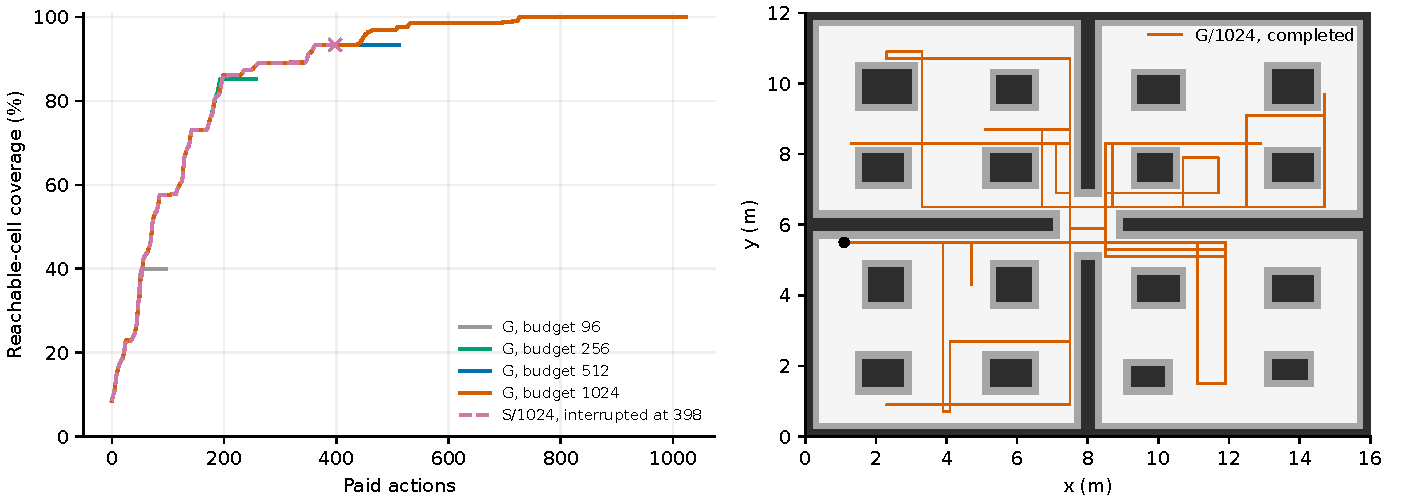
\includegraphics[width=.94\linewidth]{Four_room_budget_20261119.pdf}

\caption{Development budget diagnostics, retaining the shorter incomplete trials. The interrupted S curve ends at its last actual observation. Right: the completed G/1024 trajectory over evaluator-only geometry. Full coverage is a measured checkpoint, separate from the later return.}\label{fig:four-room-budget}\end{figure}

A separate frozen protocol compares six arms at a common 512-action cap on three generated object layouts: the inspected development layout D and two new layouts E1/E2, all sharing one four-room wall topology. Each paired set begins with an identical single sensor packet and exact pose. C scores unknown coverage; G adds measured quality and a generic structural prior; S uses category-conditioned priors; X reverses that interpretation. G2 doubles only the generic prior. S with frozen gain disables only the radar/camera posterior update while retaining fusion and directional histories. All eighteen runs are retained (Table~\ref{tab:four-room-matrix}); they represent three layouts, not eighteen independent environments.

The renderer supplies constant-gray valid RGB pixels and ideal visible category labels. Objects occupy regularly arranged slots, with no natural-image detector or measured real-world category distribution. These scenes test a synthetic planning mechanism, not realistic semantic perception. Neither the complete two-template posterior nor a trained reachability network runs in this joint variant.

Native measured-depth TSDF meshes use 6 cm voxels and 12 cm truncation. A fixed reference samples the exterior box-union boundary, excluding internal faces, and retains surfaces visible from a 0.8 m lattice of reachable camera origins. Reconstructed-area precision and fixed-reference recall at 5 cm yield surface F1~\cite{ref14}. The reference is independent of each trajectory; the supplementary protocol specifies its sampling and visibility limits.

\begin{table}[!htbp]\centering\small

\caption{All eighteen outcomes at a common 512-action cap. Entries are reachable-cell coverage / surface F1 at 5 cm, both in percent. D is development; E1/E2 are new object layouts of the same topology.}\label{tab:four-room-matrix}

\begin{tabular}{@{}lrrr@{}}\toprule Policy & D: Coverage/F1 & E1: Coverage/F1 & E2: Coverage/F1 \\ \midrule

C & 97.43/94.73 & 98.08/93.59 & 98.03/93.53 \\

G & 93.38/89.36 & 94.59/93.28 & 94.67/87.68 \\

S & 93.38/89.36 & 94.59/93.19 & 94.67/87.68 \\

X (reversed cue) & 93.91/90.09 & 94.86/93.71 & 98.03/93.13 \\

G, $2\times$ prior & 93.38/89.36 & 94.59/93.28 & 94.67/87.68 \\

S, frozen gain & 93.38/90.17 & 94.59/93.19 & 94.67/87.68 \\

\bottomrule\end{tabular}\end{table}

C exceeds G and S in both coverage and F1 on all three layouts; X also exceeds S in F1 throughout. G/S trajectories coincide in D/E2. In E1 they differ but finish with equal coverage, while S lowers F1 by 0.083 percentage points; its normalized coverage-curve area increases by only 0.000968. G2 reproduces G in all three layouts. Freezing the gain posterior improves F1 only in D, with unchanged coverage. These outcomes provide no consistent benefit from the semantic prior or gain calibration.

A post-hoc audit nevertheless distinguishes ranking from utility. For E1, four recorded S choices cannot be reproduced by any nonnegative weight in $\mathrm{common}+\lambda\,\mathrm{prior}_G$, even separately at each state, with the original cost/id tie rule. D/E2 admit uniform weights including 1 and 2. Category-conditioned ranking therefore operates in E1 without an observed endpoint benefit. On D, replay of the 98-action zero-coverage segment raises surface F1 from 88.185\% to 88.930\%: observation is useful locally but inefficient relative to the coverage control. Detailed score intervals, reference construction and replay results are retained in the supplement.

\begin{figure}[H]\centering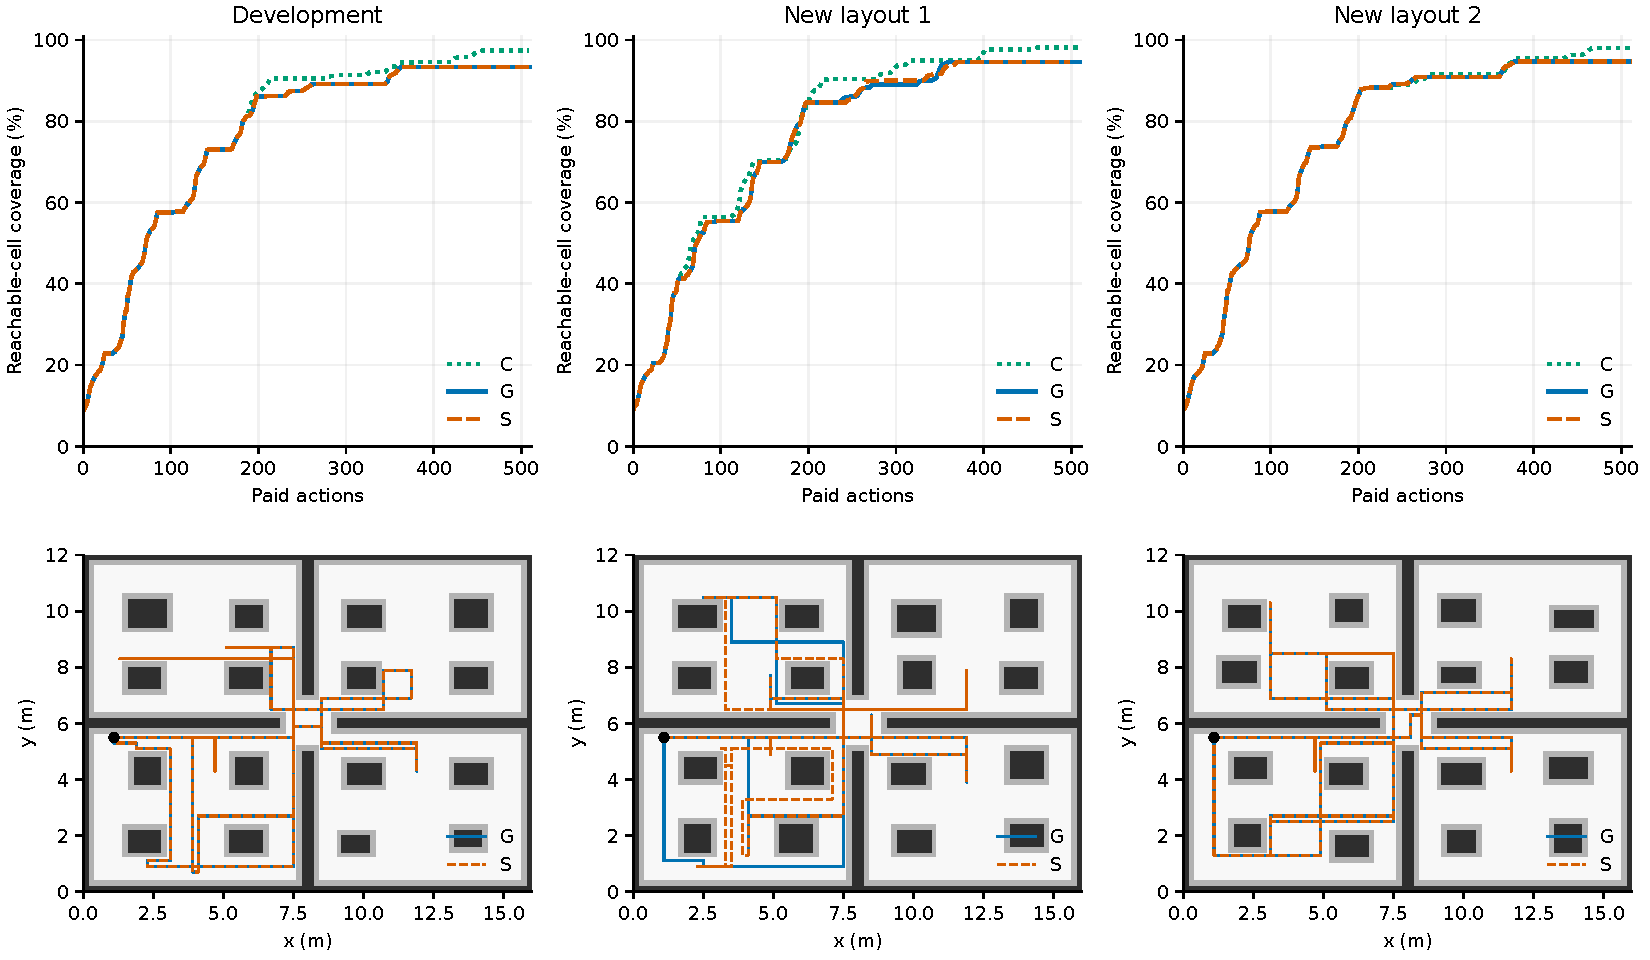
\includegraphics[width=.94\linewidth]{Four_room_matrix_20261119.pdf}

\caption{Fixed-cost coverage histories and G/S trajectories for D/E1/E2. Background geometry is evaluator-only. The full table retains the additional controls; repeated checkpoints are dependent measurements.}\label{fig:four-room-matrix}\end{figure}
